\chapter{FPGA implementations and characterisation}
\label{ch:impl&chara}

In this chapter, two \acrshort{vhdl} implementations for the ARTIX-7 \acrshort{fpga} will be proposed, based on the concept presented in the previous chapter. The feature developed for demonstrative purposes will also be presented more in-depth. Finally, a report of the \acrshort{fpga} resources usage of the BASYS-3 board that will be used for testing in the next section will be provided.\\

\section{Implementation}
\label{sec:impl}

In this section, we will first study the constraints that need to be respected to apply the proposed design to an \acrshort{fpga} implementation for ARTIX-7. This will add restrictions to the design and will lead us to two possible implementations.

Artix-7 \acrfull{clb} a made up of two slice of 4 \acrshort{lut}s, highlighted on green in figure~\ref{fig:clb_routing} and an inter-clb routing block (magenta) for the interface with the global routing of the \acrshort{fpge}. The internal routing can be programmed between \acrshort{lut}s as well.


\begin{figure}[H]
    \centering 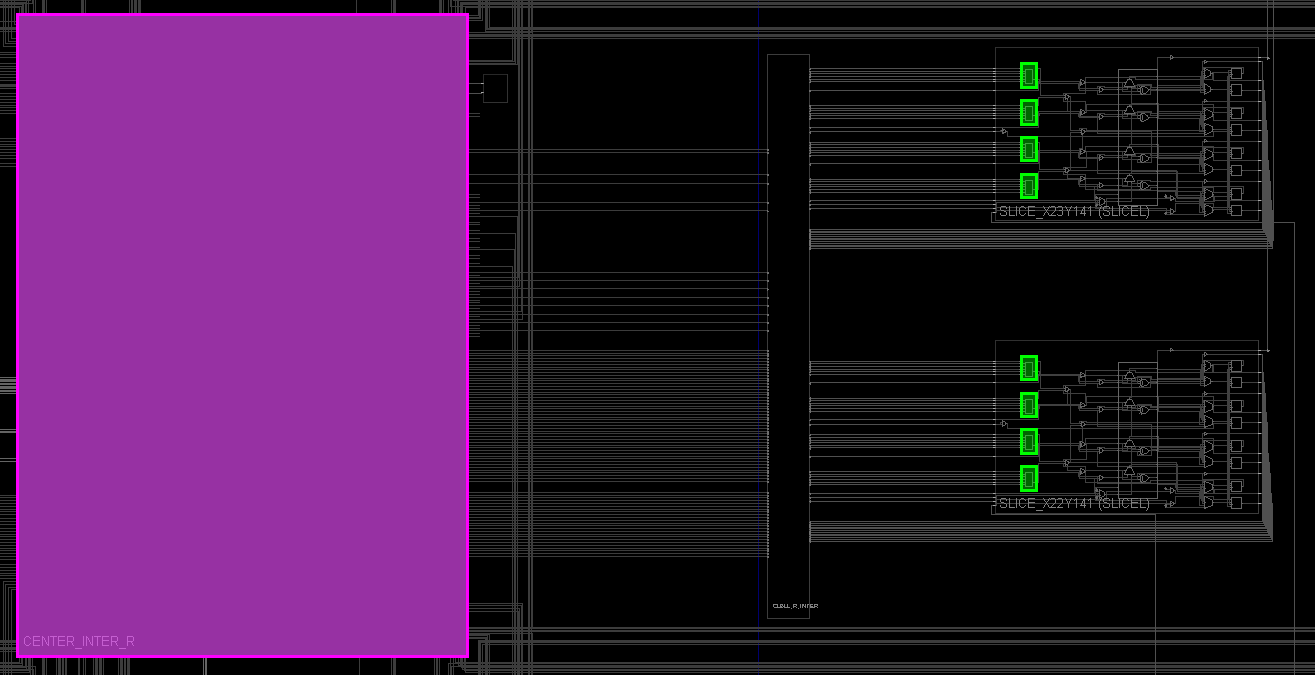
\includegraphics[width=0.9\linewidth]{images/clb_routing.png}
    \caption{Artix-7 CLB}
    \label{fig:clb_routing}
\end{figure}


\subsection{Constraints}
\label{subsec:impl_constraints}

The behaviour of the cells is very sensitive, not only to random defects in the \acrshort{ic} but to any difference both in terms of implementation (length of the loop, placement, etc...) and external factors (ageing, temperature, voltage). Therefore, to ensure that the \acrshort{puf} response is generated from the random defects with as little bias, the cell implementation should be as identical as possible. To achieve this, the \acrfull{xdc} are used to manually specify some properties of specific parts of the design.\\

By default, Vivado will try to optimise the design without changing the logical behaviour of the circuit. However, since the cell's exact behaviour is based on random defects, it can not be correctly interpreted by Vivado and any optimisation will most likely break the design. Therefore, the first constraint used is the \textbf{DONT\_TOUCH} to tell Vivado to not try to optimise the design of the cells so that it remains untouched.\\

Furthermore, the slices used to implement the cells should be the same type. On the ARTIX-7, there are two main types of slice: SLICEL (only for combinatorial functions) and SLICEM (can additionally implement memory features). There is a higher number of SLICEL available and the \acrshort{tero} cells do not need any memory functionalities. For this reason, only SLICEL are used for the PUF implementation. This is archived using \textbf{LOC} constraints.\\


The routing of the internal loop between the LUTs should also be identical. To simplify the routing management, constraining the cells to only one \acrshort{clb} could ensure that the internal loop does not need to use global routing and can stay inside the \acrshort{clb}. The \textbf{BEL} is used to fix the exact LUT used for an element and \textbf{RLOC} to place elements in slices that are next to each other. It is also possible to assign each input to a specific pin of the LUTs using \textbf{LOCK\_PINS}, to ensure an identical internal path for all the cells.\\
More details on how these \acrshort{xdc} constraints are used can be found in appendix~\ref{appendix:constraints}.\\

\subsection{Cell size}
\label{subsec:imple_cell_size}

From the routing constraints discussed previously, we know that it is preferable to use only one \acrshort{clb} to implement our cell because it removes the need for inter-\acrshort{clb} routing. On ARTIX-7, \acrshort{clb} contain two slices of 4 \acrshort{lut}s each. The design of the \acrshort{tero} cells imposes to have 2 AND gates and $2 N$ NOT gates with N being odd. This restricts our choice of the number of NOT gates to $N = \{1, 3\}$, which correspond to 4 and 8 LUTs respectively. Both cases are studied in parallel and their schematics are shown in figure~\ref{fig:tero_cell_4_&_8_diagram}. The first one will be noted TERO-4 and the second one TERO-8, due to their LUT usage.

\begin{figure}[H]
   \begin{minipage}[b]{\linewidth} 
        \centering
        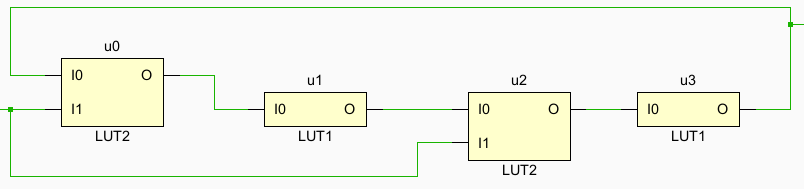
\includegraphics[width=\linewidth]{images/tero_4_schematic.png}
        \subcaption{TERO-4 (N=1)}
   \end{minipage}
   \begin{minipage}[b]{\linewidth}   
        \centering
        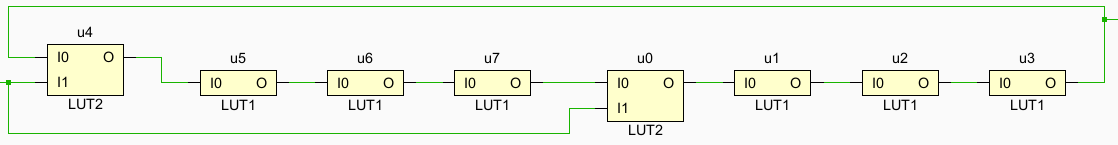
\includegraphics[width=\linewidth]{images/tero_8_schematic.png}
        \subcaption{TERO-8 (N=3)}
   \end{minipage}
   \caption{\label{fig:tero_cell_4_&_8_diagram}\acrshort{tero} cells schematics}
\end{figure}

Figure~\ref{fig:tero_8_cell_routing} represent a TERO-8 cell with the eight \acrshort{lut} in orange,  one of the internal signal is highlighted in white and the reset in green.

\begin{figure}[H]
    \centering 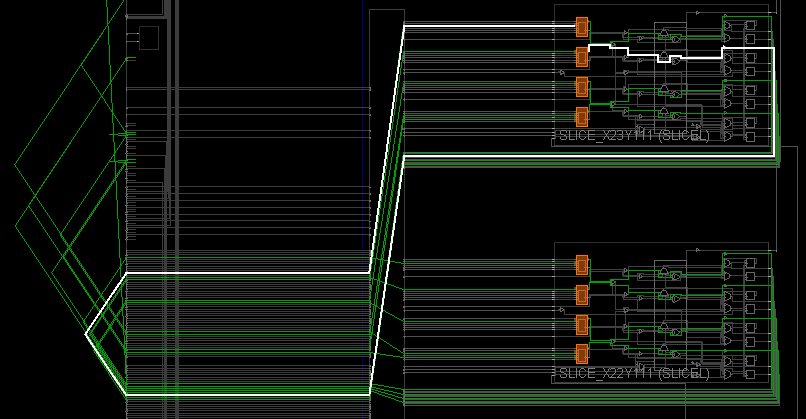
\includegraphics[width=0.9\linewidth]{images/cell_routing.png}
    \caption{TERO-8 cell routing}
    \label{fig:tero_8_cell_routing}
\end{figure}

\subsection{Number of cells}
\label{subsec:impl_number_of_cell}




\begin{minipage}[b]{0.55\linewidth} 
The initial discussion about the method to generate the response (section~\ref{sec:design_generation}) provided us with a relation between the number of cells and the response size:  $\left ( \frac{K}{2}\right )^2 -1$. The size of the PUF response needs to be high enough to be able to study their statistical properties. $2\times32$ cells are chosen here, which gives a response of 1023 bits.\\

For the implementation using TERO-8 cells, the number of slices needed is doubled but it is still possible to contain the entire implementation in a single die of the BASYS-3 board used for testing. The figure~\ref{fig:tero_8_slice_usage_overview} represents the TERO-8 cells regrouped together, with one cell (2 slices) highlighted in green. This left plenty of areas to implement other functionalities in the same device.
\end{minipage}\hfill
\begin{minipage}[b]{0.32\linewidth}   
    \centering
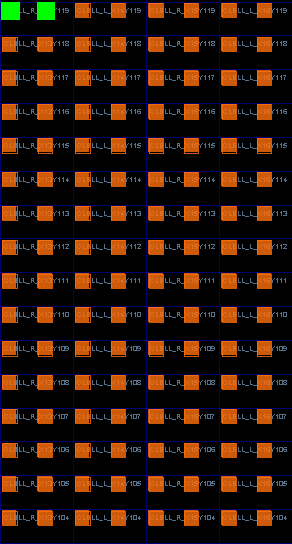
\includegraphics[width=\linewidth]{images/tero_8_array_CLB.png}
\captionof{figure}{Slices usage of TERO-8 cells arrays\label{fig:tero_8_slice_usage_overview}}
\end{minipage}

\section{Demonstrative features}
\label{sec:demon_feature}

To provide a demonstration of a security procedure using the \acrshort{tero}, some additional features are embedded in the implementation: a \acrfull{bch} decoder for error correction and a \acrshort{sha}-256 hashing function\\

\subsection{BCH decoder}
\label{subsec:demon_feature_bch}

\acrshort{ecc} are good options to improve the reliability of the response. Commonly used in applications such as satellite communication, CD-player or USB flash drive, the \acrshort{bch} code operates using helper data (called syndrome) to correct up to a certain number of random errors. It is represented using 3 parameters $BCH(N, K)$: $N$ is the size of encoded data length and $K$ is the message length. This also fixes the maximal number of errors that can be successfully corrected $T$, as well as the syndrome's size $N - K$ \cite{freudenberger_reduced_2021}.\\

The syndrome is computed beforehand from the reference response (during the provision step) and can be either stored on the device or transmitted when needed. The syndrome can be fully revealed since it does not contain any information useful to predict the original response. During the evaluation step, the response of the PUF is checked with the help of the syndrome, and as long as the number of errors is lower than $T$, it can correct them.\\

In the implementation of \cite{de_weerdt_implementation_2021}, an \acrshort{bch} decoder was added in the FPGA design, and the syndrome was computed externally (using Matlab) and then send to the device when needed. The same \acrshort{bch} implementation is used in this thesis. The parameter has been set to $BCH(255, 171)$, therefore only the first 171 bits of the PUF response are considered. This corresponds to $T=11$ correctable errors and a syndrome of 84 bits. This is enough to study the improvement in the reliability while having a moderate area usage overhead as we will see in chapter~\ref{ch:result}.\\

\begin{figure}[H]
    \centering 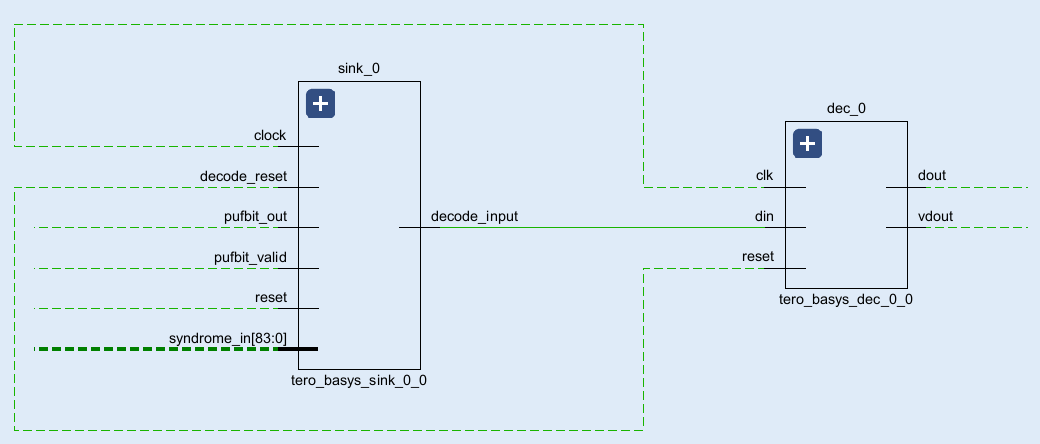
\includegraphics[width=\linewidth]{images/bch_schematic.png}
    \caption{BCH(255, 171) schematic}
    \label{fig:bch_schematic}
\end{figure}

One can notice that due to the way the cell combinations are produced by the \acrshort{lsfr}, taking only the first bits of the responses will lead to a non-uniform usage of the cells for those retained bits. This is discussed in the appendix~\ref{appendix:lsfr} where we conclude that this does not have a significant impact on the results found in the next section.



\subsection{SHA-256}
\label{subsec:demon_feature_sha}

A hashing function can be useful to transform the \acrshort{puf}'s response into a usable key for security applications. Since one goal of this study was to improve the demonstration part of the framework, it has been chosen to implement this \acrshort{sha}-256 algorithm in the \acrshort{fpga} itself.\\

There are already \acrshort{vhdl} implementations available with open-source licenses online. Therefore, it had been chosen not to re-implement those well-defined operations and to use one of these. The implementation we selected is from the GitHub repository of the user "\textbf{batiati}" \cite{batiati_vhdl_2021}. The author made available two implementations: one that operates on a single chunk of 512 bits, and the second that operates as a pipeline. We will only need to hash a single key at a time so the first implementation is sufficient.\\

The \acrshort{sha}-256 hashing operate on a block of 512 bits, that need to be padded from the original input as explained in ~\cite{technology_secure_2015}. First, the input need to be split into blocks of 447 bits maximum. To those blocks, a single \textbf{'1'} is added, and then we pad with \textbf{'0'} until the block reaches 448 bits. Finally, the 64 remaining bits are the length of the initial input (between 0 and 447) in binary form.

In our case, the input is the response of the \acrshort{bch} decoder. This always has the same size (171 bits) and fits into a single block. The corresponding padded block is represented in table~\ref{tab:sha256_padding}.\\

\begin{table}[H]
    \centering
    \begin{tabular}{|c|c|c|c|}
        \hline
        Input & Single \textbf{1} & \textbf{0} padding & Input size (64 bits)\\
        \hline
        171 bits & 1 bit & 276 bits & 64 bits\\
        \hline
        \textit{PUF after BCH} & \textbf{1} & \textbf{00..00} & \textbf{0000 ... 1010 1011} \\
        \hline
    \end{tabular}
    \caption{512 block padding for \acrshort{sha}-256}
    \label{tab:sha256_padding}
\end{table}

This gives us the complete \acrshort{sha}-256 block represented in figure~\ref{fig:sha_schematic} with first the padding block receiving bit from the \acrshort{bch} decoder, followed by the \acrshort{sha} block. It has been validated it using test vectors from the \acrfull{nist}~\cite{computer_security_division_example_2016} before adding it to the rest of our implementation.\\

\begin{figure}[H]
    \centering
    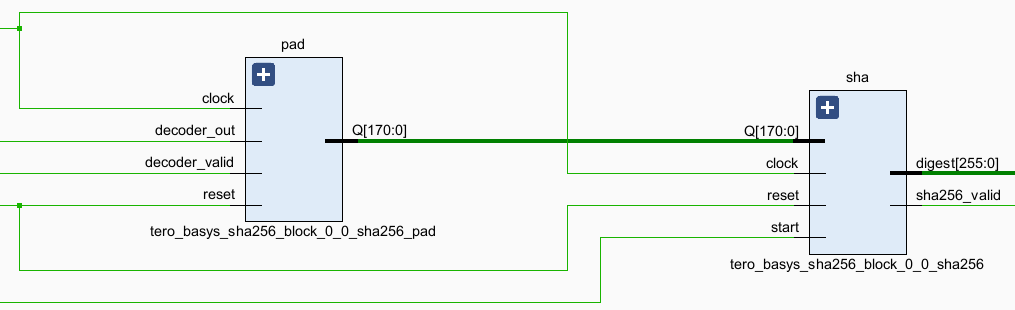
\includegraphics[width=\linewidth]{images/sha256_schematic.png}
    \caption{\acrshort{sha}-256 block schematic}
    \label{fig:sha_schematic}
\end{figure}

\section{FPGA usage}
\label{sec:fpga_usage}

We have now described all elements of our TERO PUF implementations for the ARTIX-7. The first step to characterise it is to analyse the resources used on the boards.

\subsection{Area}
\label{subsec:fpga_usage_area}

The total area usage of the implementation on a Basys-3 board can be seen in figure~\ref{fig:overview_area_usage}. The slices used for \acrshort{tero} cells are coloured orange because they have a fixed location, while the rest of the used area is light blue.

\begin{figure}[H]
    \centering
    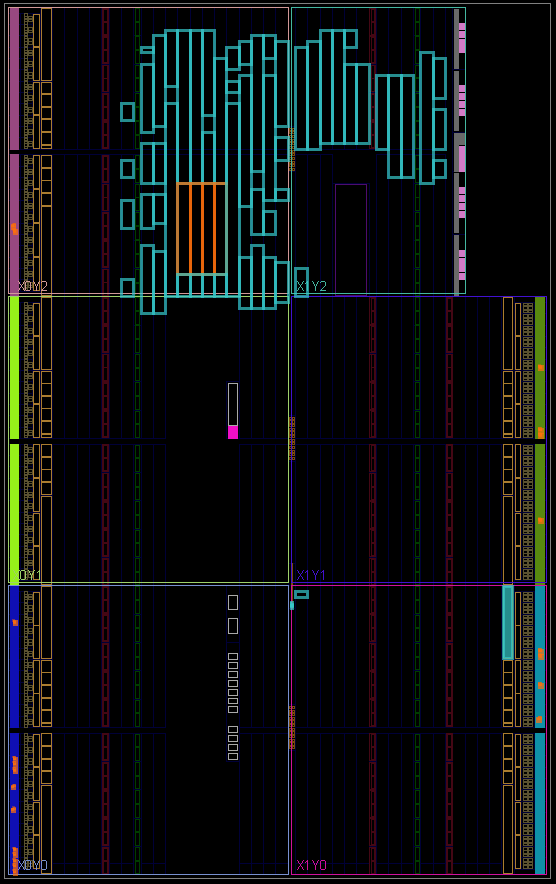
\includegraphics[width=0.65\linewidth]{images/overview_area_usage.png}
    \caption{Total area usage}
    \label{fig:overview_area_usage}
\end{figure}



The individual blocks can also be highlighted to show the placement made by Vivado. This is done on figure~\ref{fig:fpga_area_usage_detailled} for the \acrshort{puf} block (containing the cells and the elements required to generate the response), the control and \acrfull{uart} block, the \acrshort{bch} decoder and the \acrshort{sha}-256.

\begin{figure}[H]
   \begin{minipage}[b]{0.5\linewidth} 
        \centering
        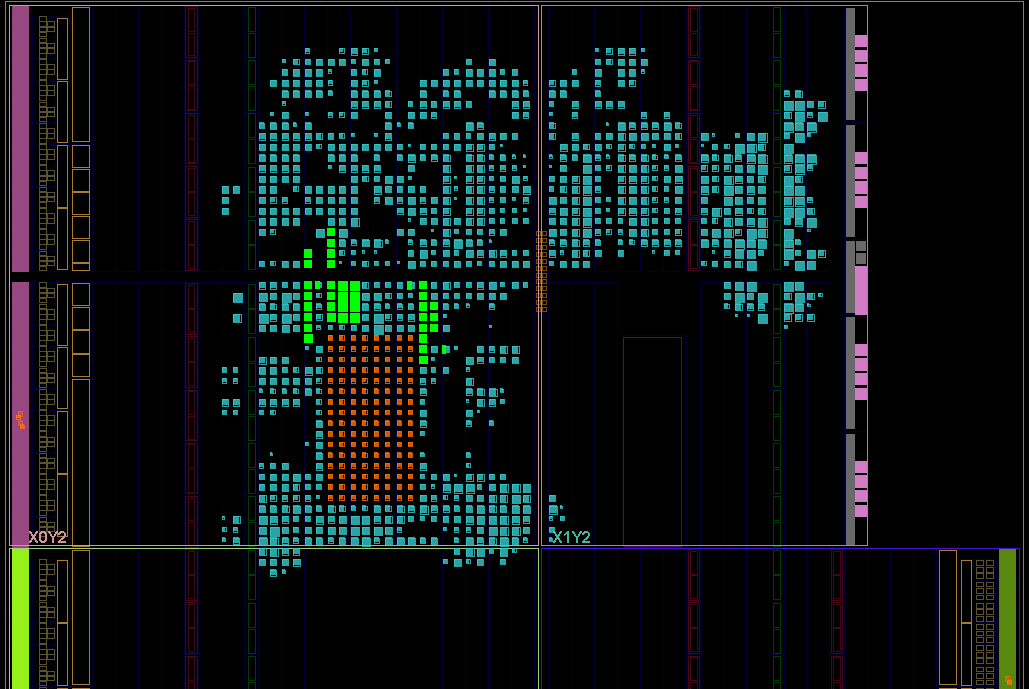
\includegraphics[width=\linewidth]{images/tero_block_area_usage.png}
        \subcaption{\acrshort{puf} block}
   \end{minipage}\hfill
   \begin{minipage}[b]{0.5\linewidth}   
        \centering
        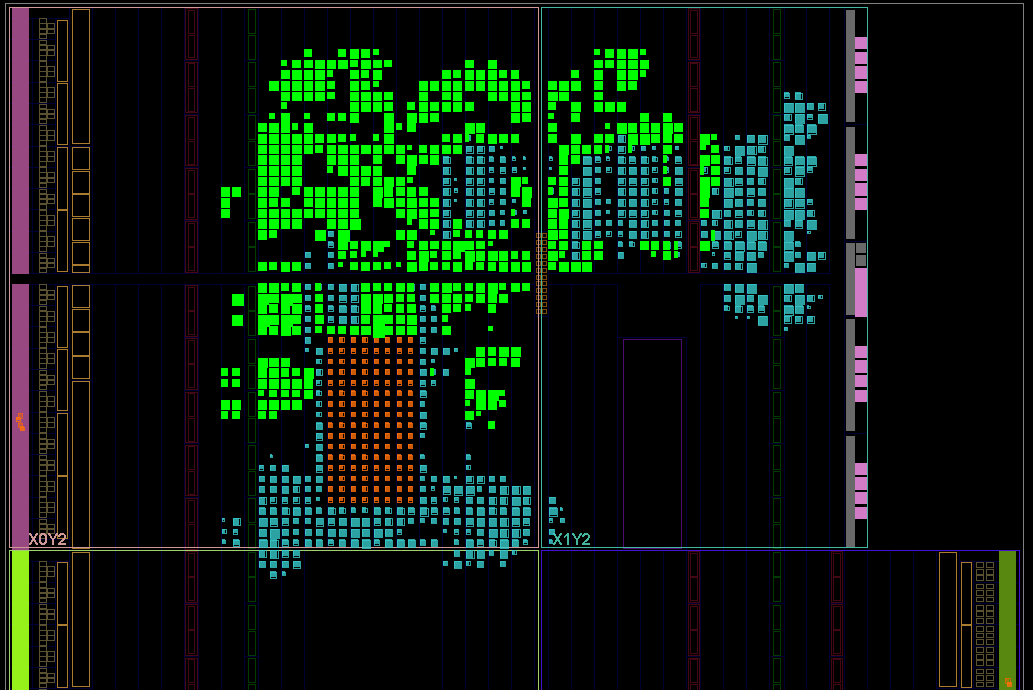
\includegraphics[width=\linewidth]{images/control_and_interface_area_usage.png}
        \subcaption{Control \& \acrshort{uart}}
   \end{minipage}
   \begin{minipage}[b]{0.5\linewidth} 
        \centering
        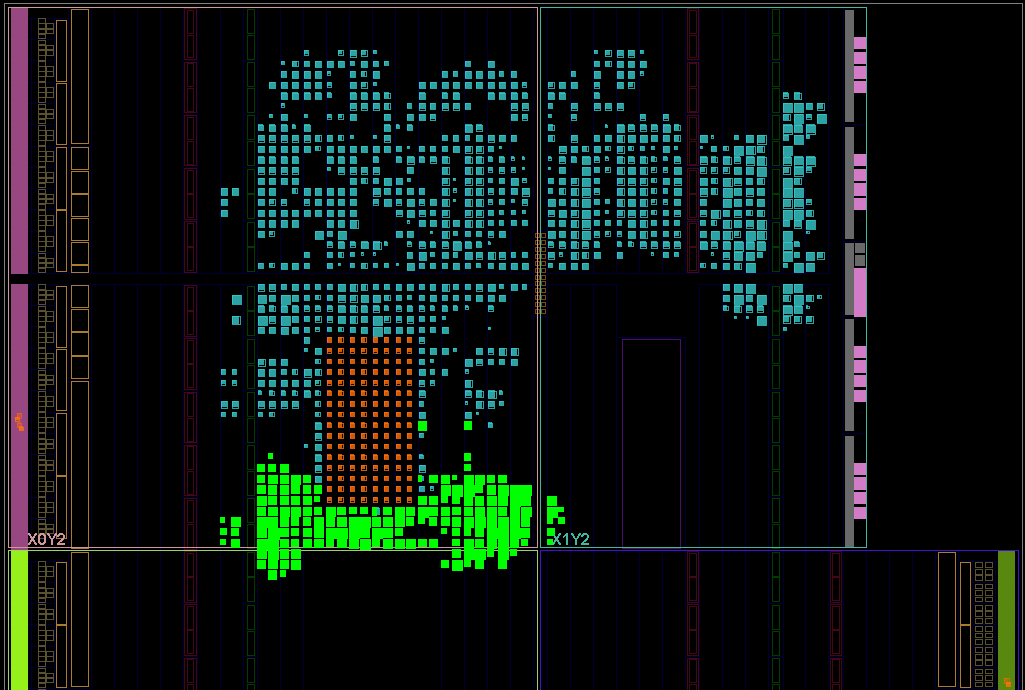
\includegraphics[width=\linewidth]{images/decoder_area_usage.png}
        \subcaption{\acrshort{bch} decoder}
   \end{minipage}\hfill
   \begin{minipage}[b]{0.5\linewidth}   
        \centering
        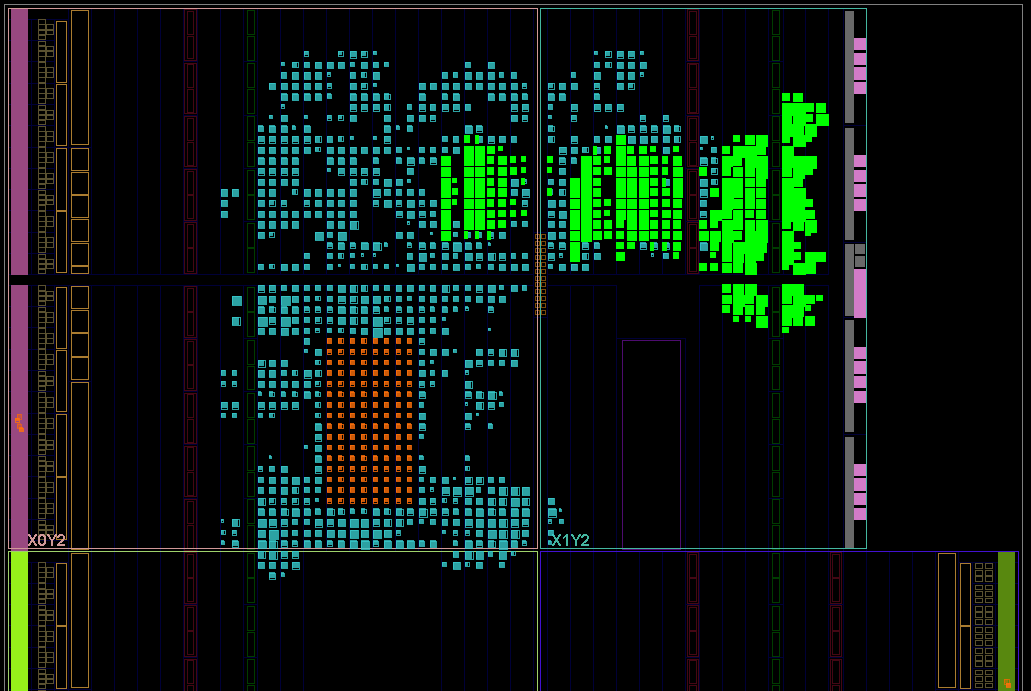
\includegraphics[width=\linewidth]{images/sha256_area_usage.png}
        \subcaption{\acrshort{sha}-256}
   \end{minipage}
   \caption{\label{fig:fpga_area_usage_detailled}Basys-3 usage per block}
\end{figure}

The primitive statistic for each part of the implementation is reported on the tables~\ref{tab:tero_4_fpga_area_usage} and \ref{tab:tero_8_fpga_area_usage}, as well as the total usage reported by Vivado.

\begin{table}[H]
    \centering
    \begin{tabular}{|l|c|c|}
         \hline
         \textbf{Primitive statistic} & \textbf{LUTs} & \textbf{Flop latches} \\
         \hline
         TERO-4 \acrshort{puf} Block & 428 | 11\% & 162 | 5\% \\
         \hline
         \acrshort{bch} decoder & 797 | 20\% & 981 | 29\%\\
         \hline
         \acrshort{sha}-256 & 895 | 23\% & 950 | 28\%\\
         \hline
         Control \& \acrshort{uart} & 1792 | 46\% & 1308 | 38\%\\       
         \hline
         Total & 3912 & 3401\\
         \hline
    \end{tabular}
    \caption{TERO-4 \acrshort{fpga} resources usage}
    \label{tab:tero_4_fpga_area_usage}
\end{table}


\begin{table}[H]
    \centering
    \begin{tabular}{|l|c|c|}
         \hline
         \textbf{Primitive statistic} & \textbf{LUTs} & \textbf{Flop latches} \\
         \hline
         TERO-8 \acrshort{puf} Block & 684 | 16\% & 162 | 5\% \\
         \hline
         \acrshort{bch} decoder & 797 | 19\% & 981 | 29\%\\
         \hline
         \acrshort{sha}-256 & 895 | 21\% & 950 | 28\%\\
         \hline
         Control \& \acrshort{uart} & 1792 | 43\% & 1308 | 38\%\\       
         \hline
         Total & 4168 & 3353\\
         \hline
    \end{tabular}
    \caption{TERO-8 \acrshort{fpga} resources usage}
    \label{tab:tero_8_fpga_area_usage}
\end{table}

The TERO-8 \acrshort{puf} block requires more resources than the TERO-4 one, which makes sense since the TERO-8 cells need twice as many slices then the TERO-4 ones. In both cases, it is the less significant part of the implementations and the control \& \acrshort{uart} takes most of the space.

\subsection{Power consumption}
\label{subsec:fpga_usage_pwr}

\begin{figure}[H]
    \centering
    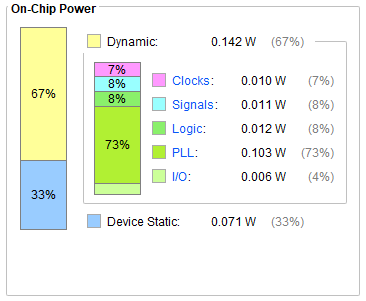
\includegraphics[width=0.7\linewidth]{images/power_usage.png}
    \caption{Power report for TERO-8}
    \label{fig:tero_8_power_usage}
\end{figure}

The power report from Vivado\ref{fig:tero_8_power_usage} indicate an estimated 0.142W of dynamic and an additional 0.071W for the static part such that the total estimated power consumption is 0.213W. We can see that the higher contribution (73\%) is the \acrfull{pll} and that the remaining parts only consume 0.039W (27\%).


